\section{Introduction}

\begin{figure}[!t]
\centering
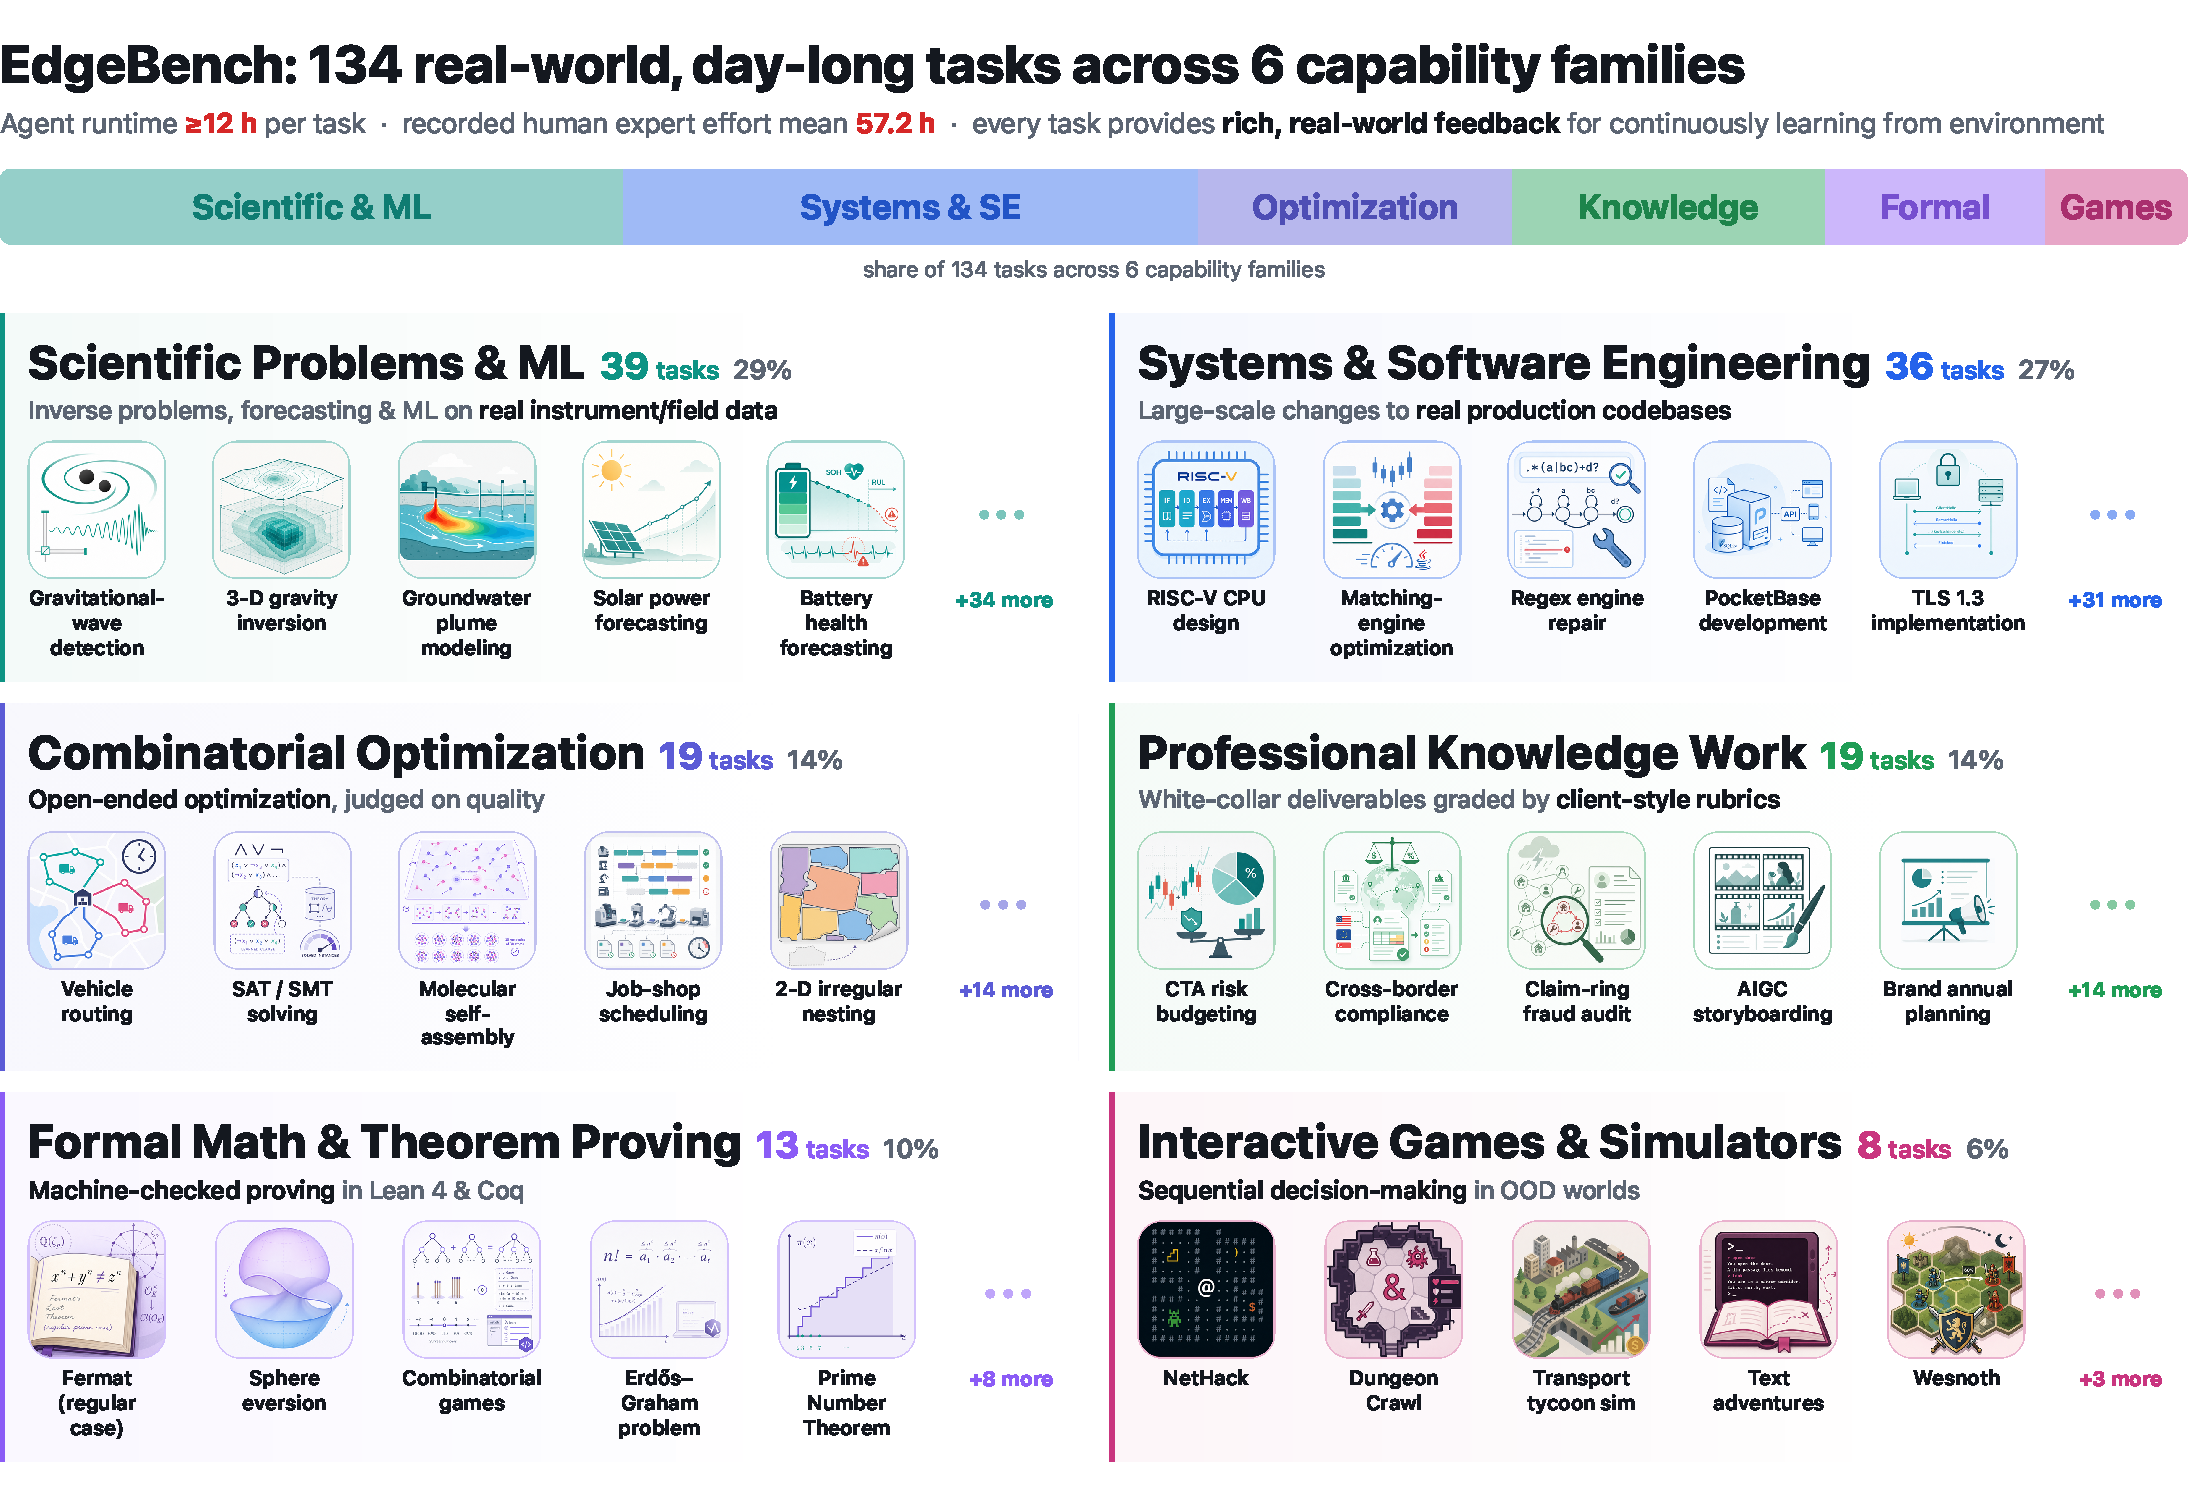
\includegraphics[width=\linewidth]{figures/edgebench_taxonomy.pdf}
\caption{\benchmark{} task taxonomy. 134 real world tasks across six capability families, with feedback channels designed to support within-run improvement. Recorded human expert effort estimates: mean 57.2 h.}
\label{fig:taxonomy}
\end{figure}

Scaling laws for pretraining~\citep{kaplan2020scaling,hoffmann2022training} revealed that model capability improves predictably with data and compute, an insight that guided much of the progress in the years that followed~\citep{openai2023gpt4,openai2025gpt45systemcard,openai2025gpt5systemcard,openai2025gpt52systemcard,openai2026gpt54thinkingsystemcard,openai2026gpt55systemcard,dubey2024llama3,anthropic2024claude35,anthropic2026claudeopus48systemcard,geminiteam2024gemini15,geminiteam2025gemini25}. Now, as large language models enter the agent era, they are being deployed into a growing range of real world environments where they can try to learn from interaction, yet whether learning from such environments obeys a clean scaling law remains unknown. Analyzing roughly 38{,}000 hours of agent environment interaction across 134 diverse real world tasks, we find, to the best of our knowledge, the first evidence that \textbf{when agents learn from real world environments, overall performance follows a log-sigmoid scaling law as a function of environment interaction time}, achieving remarkably high precision with $R^2 = 0.998$.

Why study agents' ability to learn from their environments? Real world use of AI depends on more than what a model learned during training. Some needed knowledge never appears in training data, such as private records and internal tools. Even when raw data exists, it omits the human process behind it: the trial-and-error, the interpretation of evidence, and the adaptation to feedback through which experts actually reach results. The real world also never stands still: human knowledge keeps advancing, and new tools, discoveries, and problems continually emerge that no fixed training corpus can anticipate. Therefore, an agent's ability to learn from its environment and improve task performance is central to deploying AI systems at scale in the real world.

Studying this ability requires task environments that resemble real use, provide informative feedback for learning, and allow agents enough time to learn through interaction. However, existing benchmarks often lack such feedback or limit agents to only minutes or a few hours, making them not well suited to this goal~\citep{jimenez2024swebench,chan2024mlebench,merrill2026terminalbench,sun2026agentslastexam,chu2026frontierswe,xu2026autolab}. To address this gap, we created \textbf{\benchmark{}}. Our benchmark contains \textbf{134 realistic and diverse tasks spanning six capability families}, from scientific research and software engineering to formal mathematics and interactive games, as shown in Figure~\ref{fig:taxonomy}. Each task runs in an executable workspace that combines fast local exploration with slower judge feedback on submitted artifacts, mirroring real-world workflows. Agents can work for at least \textbf{12 hours} on each task (by contrast, Agents' Last Exam~\citep{sun2026agentslastexam} averages roughly one hour per task), while we record their submissions and track how performance changes throughout the run. These tasks are substantial even for human experts: recorded expert effort averages \textbf{57.2 hours} per task and reaches up to \textbf{320 hours}. This makes \benchmark{} a natural testbed for studying how agents learn from their environments over long horizons.

Using \benchmark{}, we evaluate frontier agents over roughly 38{,}000 hours of
environment interaction. Our study makes four main observations:

\begin{itemize}
    \item \textbf{Environment learning exhibits a precise log-sigmoid scaling law.}
    Averaged performance follows the same functional form across the full
    benchmark, across task families, under longer interaction horizons up
    to 72 hours, and when forecasting later performance from early
    trajectories.

    \item \textbf{A theoretical derivation of the log-sigmoid law.}
    We propose a theory that models environment learning as a frontier expansion process on latent task graphs, which explains why benchmark-averaged progress takes the
    observed log-sigmoid form.

    \item \textbf{Agent learning speed doubles roughly every three months.}
    Studying frontier models released since September 2025, we find a rapid
    scaling trend in how quickly frontier agents learn from their environments.

    \item \textbf{Learning dynamics strongly shape long-horizon performance.}
    Long-horizon performance depends on how agents use accumulated experience,
    not only on how many attempts they make. Continuous experience outperforms
    independent restarts, longer context improves retention, and detailed
    case studies show that feedback can turn many failed probes into a few
    durable gains.
\end{itemize}
